% !TEX program = xelatex
% weekly review deck 2026-11-09 to 11-15, self-contained
\documentclass[aspectratio=169,10pt,fontset=none]{ctexbeamer}
\usepackage{fontspec}
\setCJKmainfont{Microsoft YaHei}
\setCJKsansfont{Microsoft YaHei}

\usepackage{amsmath,amssymb}
\usepackage{mathtools}
\usepackage{booktabs}
\usepackage{array}
\usepackage{colortbl}
\usepackage{graphicx}
\graphicspath{{./}{Attachments/}{../Attachments/}{../../Attachments/}{../../../Attachments/}}
\usepackage{tikz}
\usetikzlibrary{arrows.meta,positioning,calc}

% ---------- 配色（沿用库内讲义配色） ----------
\definecolor{ink}{HTML}{1F3864}
\definecolor{accent}{HTML}{C00000}
\definecolor{gold}{HTML}{BF8F00}
\definecolor{greenink}{HTML}{2E6B2E}
\definecolor{paper}{HTML}{F5F7FA}

\usetheme{default}
\usecolortheme[named=ink]{structure}
\setbeamertemplate{navigation symbols}{}
\setbeamertemplate{itemize items}[circle]
\setbeamercolor{structure}{fg=ink}
\setbeamercolor{frametitle}{fg=ink}
\setbeamercolor{block title}{bg=ink!12,fg=ink}
\setbeamercolor{block body}{bg=ink!4,fg=black}
\setbeamercolor{block title alerted}{bg=accent!12,fg=accent}
\setbeamercolor{block body alerted}{bg=accent!4,fg=black}
\setbeamercolor{block title example}{bg=greenink!14,fg=greenink}
\setbeamercolor{block body example}{bg=greenink!5,fg=black}
\setbeamerfont{frametitle}{size=\large,series=\bfseries}
\setbeamerfont{footline}{size=\scriptsize}
\addtobeamertemplate{block begin}{\vspace{-2.5pt}}{}
\addtobeamertemplate{block end}{}{\vspace{-2.5pt}}
\addtobeamertemplate{block alerted begin}{\vspace{-2.5pt}}{}
\addtobeamertemplate{block alerted end}{}{\vspace{-2.5pt}}
\addtobeamertemplate{block example begin}{\vspace{-2.5pt}}{}
\addtobeamertemplate{block example end}{}{\vspace{-2.5pt}}
\setbeamertemplate{frametitle}{\vskip3pt\insertframetitle\par\vskip1.5pt%
  \textcolor{accent}{\rule{\textwidth}{0.7pt}}\vskip-3pt}
\setbeamertemplate{footline}{%
  \hbox to \paperwidth{\hspace{8pt}%
    \textcolor{ink!55}{本周 Daily Exercise 回顾\ \ ·\ \ 11-09 -- 11-15\ \ ·\ \ 42 题详解版}\hfill
    \textcolor{ink!55}{\insertframenumber\,/\,\inserttotalframenumber}\hspace{9pt}}\vskip5pt}
\setbeamersize{text margin left=0.75cm,text margin right=0.75cm}
\setlength{\parindent}{0pt}
\setlength{\parskip}{2pt}
\AtBeginDocument{%
  \setlength{\abovedisplayskip}{3pt}\setlength{\belowdisplayskip}{3pt}%
  \setlength{\abovedisplayshortskip}{2pt}\setlength{\belowdisplayshortskip}{2pt}}

% 题号标记
\newcommand{\ex}[1]{\textcolor{accent}{\footnotesize\bfseries #1}}
\newcommand{\key}[1]{\textcolor{ink}{\bfseries #1}}

\hypersetup{pdftitle={本周 Daily Exercise 回顾（2026-11-09 至 11-15，42 题详解版）},
  pdfsubject={Artin Algebra 2e, Ch. 3--6 random review and Ch. 8 Sections 2--4: 42 exercises weekly review},
  pdfauthor={exercise\_abstract}}
\title{本周 Daily Exercise 回顾（2026-11-09 至 11-15，42 题详解版）}
\author{exercise\_abstract}

\begin{document}
% ============================================================ 1 标题页
\begin{frame}[plain]
\pdfbookmark[1]{封面}{bm:cover}
  \begin{tikzpicture}[remember picture,overlay]
    \fill[ink] (current page.north west) rectangle ([yshift=-4.75cm]current page.north east);
    \node[anchor=north west,text=white,font=\fontsize{25}{29}\selectfont\bfseries]
      at ([xshift=1.0cm,yshift=-0.92cm]current page.north west) {本周 Daily Exercise 回顾};
    \node[anchor=north west,text=white!90]
      at ([xshift=1.02cm,yshift=-2.08cm]current page.north west)
      {\large 覆盖 2026-11-09 -- 11-15（7 份清单，42 题）\quad·\quad 逐题详解版};
    \node[anchor=north west,text=white!75]
      at ([xshift=1.02cm,yshift=-2.86cm]current page.north west)
      {\small Artin \textit{Algebra} 2e：Ch.~3--6 复习抽查 + Ch.~8 \S2--\S4 系统推进\quad·\quad 线代 37 + 群论 3 + 域论 2\quad·\quad 难度 19/18/5};
    \node[anchor=north east,text=white!60,font=\small]
      at ([xshift=-1.0cm,yshift=-0.92cm]current page.north east) {exercise\_abstract};
    \node[anchor=west,text=white!55,font=\tiny]
      at ([xshift=1.02cm,yshift=-4.45cm]current page.north west)
      {数据来源：\texttt{10 - Daily Exercise Lists} 的 7 份清单；题面与来源取自 42 篇习题笔记并经原书 PDF 核对；数学结论经独立复核与程序验算；快照 2026-11-15};
  \end{tikzpicture}
  \vspace*{4.9cm}
  \begin{columns}[T,onlytextwidth]
    \begin{column}{0.50\textwidth}
      \begin{block}{两条主线（本周清单的两区）}
        \scriptsize
        \begin{itemize}\setlength{\itemsep}{1pt}
          \item \key{Random Review（21 题，Ch.~3--6 复习抽查）}\\
                子域与四元矩阵域、$\ell^p$ 空间、基与维数、秩零化度与单侧逆、特征多项式与 Jordan 型、旋转矩阵与共轭连续性、$GL_2/SL_2$ 阶、八面体极点轨道、超立方体对称群、六重点群壁纸群
          \item \key{Systematic Progress（21 题，Ch.~8 \S2--\S4，LA202--LA222）}\\
                正定矩阵的性质与运算、Hermite 型的实虚部与基、Gram 矩阵、正交列求逆、投影与 Gram--Schmidt、Legendre 多项式、Frobenius 内积、正交补恒等式、迹型的符号差
        \end{itemize}
      \end{block}
    \end{column}
    \begin{column}{0.47\textwidth}
      \begin{block}{这一版的用法与边界}
        \scriptsize
        \begin{itemize}\setlength{\itemsep}{1pt}
          \item 每题：完整题面 → 一句思路 → \textbf{显示中间式的推导} → 具体验算/反例
          \item 7 份清单全部存在（11-09 至 11-15 逐日生成），共 42 题，互不重复
          \item 这是\textbf{快照}：题单若之后追加，以库内文件为准
          \item 计算型结论经 NumPy 独立验算（14 项全部通过）；LA148 的原书符号问题按两种读法分别报告
          \item 第 \pageref{sec:answers} 页起是 42 题速查表、方法卡、易错点与自测
        \end{itemize}
      \end{block}
    \end{column}
  \end{columns}
\end{frame}

% ============================================================ 2 本周概览
\begin{frame}[t]{一、本周概览：7 份题单、42 题、两个独立队列}
  \label{sec:overview}
\pdfbookmark[1]{一、本周概览}{bm:sec-overview}
  \centering
  \scriptsize
  \setlength{\tabcolsep}{3pt}
  \renewcommand{\arraystretch}{1.14}
  \begin{tabular}{@{}l l l@{}}
    \toprule
    日期 & Random Review（3 题） & Systematic Progress（3 题）\\
    \midrule
    11-09（一） & F28，LA163，LA148 & LA205，LA206，LA207\\
    11-10（二） & LA97，LA140，LA158 & LA202，LA203，LA204\\
    11-11（三） & LA118，F29，LA77 & LA208，LA209，LA210\\
    11-12（四） & LA183，LA167，LA93 & LA214，LA215，LA216\\
    11-13（五） & LA149，LA105，LA90 & LA211，LA212，LA213\\
    \rowcolor{ink!7} 11-14（六） & G182，LA79，G190 & LA217，LA218，LA219\\
    \rowcolor{ink!7} 11-15（日） & LA134，LA145，G152 & LA220，LA221，LA222\\
    \midrule
    合计 & \textbf{21} 题（Ch.~3--6） & \textbf{21} 题（Ch.~8 \S2--\S4）\\
    \bottomrule
  \end{tabular}
  \vspace{0.35em}
  \raggedright
  \begin{columns}[T,onlytextwidth]
    \begin{column}{0.49\textwidth}
      \begin{exampleblock}{\footnotesize 数据观察}
        \scriptsize
        \begin{itemize}\setlength{\itemsep}{1pt}
          \item \textbf{7 天题单齐全}：11-09 至 11-15 每天两区各 3 题，本周无缺日；42 题互不重复。
          \item 系统区本周按清单日期呈现 \S3 $\to$ \S2 $\to$ \S3 $\to$ \S4 的推进顺序，覆盖 Ex.~2.1--4.13 中的 21 题；随机区为 Ch.~3--6 的分层抽查。
          \item Random 与 Systematic 是两条独立队列；随机区抽题不推进系统进度，本讲义也不改动任何学习状态。
        \end{itemize}
      \end{exampleblock}
    \end{column}
    \begin{column}{0.49\textwidth}
      \begin{block}{\footnotesize 难度、来源与快照}
        \scriptsize
        \begin{itemize}\setlength{\itemsep}{1pt}
          \item 难度分布：beginner 19 / intermediate 18 / advanced 5；题材：线代 37、群论 3（G152，G182，G190）、域论 2（F28，F29）。
          \item 全部 42 题源自 Artin \textit{Algebra} 2e，笔记内均已记录 printed/PDF 双页码；本讲义逐帧标注。
          \item 快照读取于 2026-11-15；笔记 \texttt{status} 未被本任务改动。
        \end{itemize}
      \end{block}
    \end{column}
  \end{columns}
\end{frame}

% ============================================================ Random Review
\begin{frame}[t]{二、Random Review 逐题详解：F28}
\pdfbookmark[1]{二、Random Review}{bm:sec-random}
  \leavevmode\ex{F28 · Ch.~3 §1 Ex.~1.1 · printed p.~98 / PDF p.~110 · beginner}
  \pdfbookmark[2]{F28 · Ch.3 S 1 Ex~1.1}{bm:f28}
  \begin{block}{\footnotesize 题面}
    \scriptsize Prove that the numbers of the form $a+b\sqrt2$, where $a,b\in\mathbb Q$, form a subfield of $\mathbb C$.
  \end{block}
  \begin{exampleblock}{\footnotesize 思路：闭包逐条验证，逆元有理化分母}
    \scriptsize
    集合含 $0,1$，且 $(a+b\sqrt2)+(c+d\sqrt2)=(a+c)+(b+d)\sqrt2$、$(a+b\sqrt2)(c+d\sqrt2)=(ac+2bd)+(ad+bc)\sqrt2$，故加、乘、取负封闭。若 $a+b\sqrt2\ne0$，则 $a^2-2b^2\ne0$：当 $b\ne0$ 时取等会使 $\sqrt2=a/b\in\mathbb Q$，矛盾；当 $b=0$ 时迫使 $a=0$。于是
    $(a+b\sqrt2)^{-1}=\frac{a-b\sqrt2}{a^2-2b^2}$
    仍具同一形式，故非零元可逆，子域成立。$\square$
  \end{exampleblock}
  \begin{block}{\footnotesize 验算}
    \scriptsize 取 $(1+\sqrt2)^{-1}=\sqrt2-1=-1+1\cdot\sqrt2$，确为 $a,b\in\mathbb Q$ 的形式；乘回 $(1+\sqrt2)(\sqrt2-1)=1$。
  \end{block}
\end{frame}

\begin{frame}[t]{二、Random Review：LA163}
  \leavevmode\ex{LA163 · Ch.~5 §1 Ex.~1.1 · printed p.~150 / PDF p.~162 · intermediate}
  \pdfbookmark[2]{LA163 · Ch.5 S 1 Ex~1.1}{bm:la163}
  \begin{block}{\footnotesize 题面}
    \scriptsize Determine the matrices that represent the rotations of $\mathbb R^3$: (a)~angle $\theta$, axis $e_2$; (b)~angle $2\pi/3$, axis $(1,1,1)^t$; (c)~angle $\pi/2$, axis $(1,1,0)^t$.
  \end{block}
  \begin{exampleblock}{\footnotesize 思路：归一化轴向量 $u$，代入 Rodrigues 公式 $R=cI+(1-c)uu^t+s[u]_\times$}
    \scriptsize
    (a) $u=e_2$ 直接展开：$R=\begin{pmatrix}\cos\theta&0&\sin\theta\\0&1&0\\-\sin\theta&0&\cos\theta\end{pmatrix}$。
    (b) $u=(1,1,1)^t/\sqrt3$，$c=-\tfrac12$，$s=\tfrac{\sqrt3}2$：
    $$R=\begin{pmatrix}0&0&1\\1&0&0\\0&1&0\end{pmatrix},\qquad e_1\mapsto e_2\mapsto e_3\mapsto e_1.$$
    (c) $u=(1,1,0)^t/\sqrt2$，$c=0$，$s=1$：
    $$R=\begin{pmatrix}\tfrac12&\tfrac12&\tfrac1{\sqrt2}\\\tfrac12&\tfrac12&-\tfrac1{\sqrt2}\\-\tfrac1{\sqrt2}&\tfrac1{\sqrt2}&0\end{pmatrix}.$$
  \end{exampleblock}
  \begin{block}{\footnotesize 验算（NumPy 通过）}
    \scriptsize 三个矩阵均满足 $RR^t=I$、$\det R=1$，且各自固定所给轴向量。
  \end{block}
\end{frame}

\begin{frame}[t]{二、Random Review：LA148}
  \leavevmode\ex{LA148 · Ch.~4 §7 Ex.~7.4 · printed p.~129 / PDF p.~141 · advanced}
  \pdfbookmark[2]{LA148 · Ch.4 S 7 Ex~7.4}{bm:la148}
  \begin{block}{\footnotesize 题面}
    \scriptsize (a)~Determine all Jordan forms with characteristic polynomial $(t+2)^2(t-5)^3$. (b)~The printed exercise asks for the possibilities when the space of eigenvectors with eigenvalue $2$ is one-dimensional and the eigenspace for $5$ is two-dimensional.
  \end{block}
  \begin{alertblock}{\footnotesize Source issue：印刷本 (b) 写特征值 $2$，与 $(t+2)^2(t-5)^3$ 矛盾}
    \scriptsize 按字面读：$2$ 不是特征根，$2$-特征空间维数为 $0$，这样的矩阵不存在。按意图读（$-2$）：特征空间一维 $\Rightarrow$ $-2$ 恰有一个块 $J_2(-2)$；$5$-特征空间二维 $\Rightarrow$ 两个块，大小 $2+1$。唯一答案为 $J_2(-2)\oplus J_2(5)\oplus[5]$。两种读法均报告，不静默改题。
  \end{alertblock}
  \begin{exampleblock}{\footnotesize (a) 推导：块大小 = 代数重数的分拆；特征空间维数 = 块数}
    \scriptsize
    $-2$ 的分拆：$2$，$1+1$；$5$ 的分拆：$3$，$2+1$，$1+1+1$。共 $2\times3=6$ 个：
    $$J_2(-2)\oplus J_3(5),\quad J_2(-2)\oplus J_2(5)\oplus[5],\quad J_2(-2)\oplus[5]^{\oplus3},$$
    $$[-2]^{\oplus2}\oplus J_3(5),\quad [-2]^{\oplus2}\oplus J_2(5)\oplus[5],\quad [-2]^{\oplus2}\oplus[5]^{\oplus3}.$$
  \end{exampleblock}
  \begin{block}{\footnotesize 验算（NumPy 通过）}
    \scriptsize 对意图答案验证特征多项式：$\det(tI-J)$ 的根恰为 $\{-2,-2,5,5,5\}$。
  \end{block}
\end{frame}

\begin{frame}[t]{二、Random Review：LA97}
  \leavevmode\ex{LA97 · Ch.~3 §6 Ex.~6.3 · printed p.~101 / PDF p.~113 · intermediate}
  \pdfbookmark[2]{LA97 · Ch.3 S 6 Ex~6.3}{bm:la97}
  \begin{block}{\footnotesize 题面}
    \scriptsize For every positive integer $p$, let $\ell^p$ be the space of sequences $(a_i)$ such that $\sum_i|a_i|^p<\infty$. Prove that $\ell^p$ is a proper subspace of $\ell^{p+1}$.
  \end{block}
  \begin{exampleblock}{\footnotesize 思路：可和序列趋于 $0$，尾段 $|a_i|\le1$ 时指数升高只会变小}
    \scriptsize
    若 $(a_i)\in\ell^p$，则 $a_i\to0$，故充分大的 $i$ 有 $|a_i|\le1$，从而
    $$|a_i|^{p+1}\le|a_i|^p;$$
    剩余有限项不影响收敛，故 $(a_i)\in\ell^{p+1}$；包含映射显然线性。严格性：取 $a_i=i^{-1/p}$，则
    $$\sum_i|a_i|^p=\sum_i\frac1i=\infty,\qquad \sum_i|a_i|^{p+1}=\sum_i i^{-1-1/p}<\infty,$$
    后一级数是收敛的 $p$-级数（指数 $1+\tfrac1p>1$）。故 $\ell^p\subsetneq\ell^{p+1}$。$\square$
  \end{exampleblock}
  \begin{block}{\footnotesize 边界}
    \scriptsize 关键用到「可和 $\Rightarrow$ 趋于 $0$」；反例序列在 $\ell^{p+1}\setminus\ell^p$ 中，两端都不能放宽。
  \end{block}
\end{frame}

\begin{frame}[t]{二、Random Review：LA140 与 LA118（两道一行证明）}
  \leavevmode\ex{LA140 · Ch.~4 §6 Ex.~6.7 · printed p.~129 / PDF p.~141 · beginner}\quad
  \pdfbookmark[2]{LA140 · Ch.4 S 6 Ex~6.7}{bm:la140}
  \ex{LA118 · Ch.~4 §4 Ex.~4.3 · printed p.~127 / PDF p.~139 · beginner}
  \begin{block}{\footnotesize 题面}
    \scriptsize \textbf{LA140：}If $A,B$ are $n\times n$ and $A$ is nonsingular, prove that $AB$ is similar to $BA$.\\
    \textbf{LA118：}If $W_1,W_2$ are $T$-invariant subspaces of $V$, prove that $W_1+W_2$ and $W_1\cap W_2$ are $T$-invariant.
  \end{block}
  \begin{exampleblock}{\footnotesize 思路与推导}
    \scriptsize
    \textbf{LA140（共轭）：}直接计算
    $$A^{-1}(AB)A=(A^{-1}A)BA=BA,$$
    $A$ 可逆，故这是合法的相似变换，$AB\sim BA$。$\square$\\[3pt]
    \textbf{LA118（逐元素检验）：}对 $w_i\in W_i$，
    $$T(w_1+w_2)=Tw_1+Tw_2\in W_1+W_2;$$
    对 $w\in W_1\cap W_2$，不变性分别给出 $Tw\in W_1$ 与 $Tw\in W_2$，故 $Tw\in W_1\cap W_2$。$\square$
  \end{exampleblock}
  \begin{block}{\footnotesize 验算与边界}
    \scriptsize LA140 的可逆性不可去：一般 $AB$ 与 $BA$ 仅在非零特征值（含重数）上一致，未必相似。LA118 的逆命题不成立：$W_1+W_2$ 与 $W_1\cap W_2$ 不变不能推出 $W_1,W_2$ 各自不变。
  \end{block}
\end{frame}

\begin{frame}[t]{二、Random Review：LA158}
  \leavevmode\ex{LA158 · Ch.~4 Misc.\ Ex.~M.5 · printed p.~130 / PDF p.~142 · advanced}
  \pdfbookmark[2]{LA158 · Ch.4 Misc.\ Ex~M.5}{bm:la158}
  \begin{block}{\footnotesize 题面}
    \scriptsize Let $\varphi:F^n\to F^m$ be left multiplication by an $m\times n$ matrix $A$. (a)~Prove equivalence of: $A$ has a right inverse $B$ with $AB=I$; $\varphi$ is surjective; $\operatorname{rank}A=m$. (b)~Prove equivalence of: $A$ has a left inverse $B$ with $BA=I$; $\varphi$ is injective; $\operatorname{rank}A=n$.
  \end{block}
  \begin{exampleblock}{\footnotesize 思路：右逆 = 为每个 $e_j$ 选原像；左逆 = 在像上取逆再线性扩张}
    \scriptsize
    \textbf{(a)} 若 $AB=I_m$，则任意 $y=A(By)$，$\varphi$ 满；满 $\Leftrightarrow\dim\operatorname{im}A=m$。反之若 $A$ 满，取 $b_j$ 使 $Ab_j=e_j$，以诸 $b_j$ 为列作 $B$，则 $AB=I_m$。\\[2pt]
    \textbf{(b)} 若 $BA=I_n$，则 $Ax=0\Rightarrow x=BAx=0$，$\varphi$ 单；秩零化度使单 $\Leftrightarrow$ 秩 $n$。反之若 $A$ 单，在 $\operatorname{im}A$ 上定义 $B(Ax)=x$（良定，因单），将 $\operatorname{im}A$ 的基扩张为 $F^m$ 的基，在新增基向量上任意定义（如取 $0$），线性扩张得 $BA=I_n$。$\square$
  \end{exampleblock}
  \begin{block}{\footnotesize 验算与边界}
    \scriptsize 例：$A=(1\ 0):F^1\to F^2$ 有右逆 $\binom10$，秩 $1=m$；$A=\binom10:F^2\to F^1$ 有左逆 $(1\ 0)$，秩 $1=n$。方阵时两者重合（可逆）。扩张步骤用到基扩张定理，是本节的标准工具。
  \end{block}
\end{frame}

\begin{frame}[t]{二、Random Review：F29}
  \leavevmode\ex{F29 · Ch.~3 §1 Ex.~1.10 · printed p.~99 / PDF p.~111 · intermediate}
  \pdfbookmark[2]{F29 · Ch.3 S 1 Ex~1.10}{bm:f29}
  \begin{block}{\footnotesize 题面}
    \scriptsize Over $\mathbb F_2$, prove that the four matrices $0,\ I,\ A=\begin{pmatrix}1&1\\1&0\end{pmatrix},\ B=\begin{pmatrix}0&1\\1&1\end{pmatrix}$ form a field.
  \end{block}
  \begin{exampleblock}{\footnotesize 思路：识别 $B=A+I$ 与 $A^2=A+I$，乘法结构由 $A$ 的多项式给出}
    \scriptsize
    集合即 $\{0,I,A,A+I\}$，加法封闭（特征 $2$）。直接相乘（模 $2$）：
    $$A^2=\begin{pmatrix}0&1\\1&1\end{pmatrix}=A+I=B,\qquad A^3=A\cdot A^2=A(A+I)=A^2+A=I,$$
    故 $A^{-1}=A^2=B$，$B^{-1}=A$，乘法封闭。结合律、分配律继承自 $M_2(\mathbb F_2)$；每个元素都是 $A$ 的多项式，故乘法交换。四元素、非零元皆可逆 $\Rightarrow$ 是域，同构于 $\mathbb F_2[x]/(x^2+x+1)$。$\square$
  \end{exampleblock}
  \begin{block}{\footnotesize 验算（NumPy 模 2 通过）}
    \scriptsize 程序验证 $A^2\equiv A+I$、$A^3\equiv I\pmod 2$；加法表为 Klein 四群，非零元乘法为 3 阶循环群 $\{I,A,A^2\}$。
  \end{block}
\end{frame}

\begin{frame}[t]{二、Random Review：LA77 与 LA93}
  \leavevmode\ex{LA77 · Ch.~3 §2 Ex.~2.1 · printed p.~99 / PDF p.~111 · beginner}\quad
  \pdfbookmark[2]{LA77 · Ch.3 S 2 Ex~2.1}{bm:la77}
  \ex{LA93 · Ch.~3 §5 Ex.~5.2 · printed p.~100 / PDF p.~112 · beginner}
  \begin{block}{\footnotesize 题面}
    \scriptsize \textbf{LA77：}(a)~Prove $0v=$ zero vector; (b)~if $w\in W$ then $-w\in W$.\\
    \textbf{LA93：}Let $W_1$ be the trace-zero real $n\times n$ matrices. Find $W_2$ with $\mathbb R^{n\times n}=W_1\oplus W_2$.
  \end{block}
  \begin{exampleblock}{\footnotesize 思路与推导}
    \scriptsize
    \textbf{LA77(a)（加群消去）：}
    $$0v=(0+0)v=0v+0v\ \Longrightarrow\ 0v=0.$$
    \textbf{LA77(b)（标量闭包）：}$(-1)w\in W$，且 $w+(-1)w=(1-1)w=0w=0$，故 $(-1)w=-w\in W$。$\square$\\[3pt]
    \textbf{LA93（取 $W_2=\mathbb RI$）：}每个 $A$ 有分解
    $$A=\Big(A-\frac{\operatorname{tr}A}{n}I\Big)+\frac{\operatorname{tr}A}{n}I,\qquad \operatorname{tr}\Big(A-\frac{\operatorname{tr}A}{n}I\Big)=\operatorname{tr}A-\operatorname{tr}A=0;$$
    若 $cI\in W_1$ 则 $0=\operatorname{tr}(cI)=cn$ 得 $c=0$，交为零，故为直和。$\square$
  \end{exampleblock}
  \begin{block}{\footnotesize 验算}
    \scriptsize LA93 取 $n=2$、$A=\mathrm{diag}(3,-1)$：$A=(\mathrm{diag}(2,-2))+1\cdot I$，迹 $0+2=2=\operatorname{tr}A$。补空间不唯一，但 $\mathbb RI$ 最自然。
  \end{block}
\end{frame}

\begin{frame}[t]{二、Random Review：LA183 与 LA105}
  \leavevmode\ex{LA183 · Ch.~5 §4 Ex.~4.8 · printed p.~152 / PDF p.~164 · beginner}\quad
  \pdfbookmark[2]{LA183 · Ch.5 S 4 Ex~4.8}{bm:la183}
  \ex{LA105 · Ch.~4 §1 Ex.~1.3 · printed p.~125 / PDF p.~137 · beginner}
  \begin{block}{\footnotesize 题面}
    \scriptsize \textbf{LA183：}If $B_k\to B$ and $P$ is invertible, prove $P^{-1}B_kP\to P^{-1}BP$.\\
    \textbf{LA105：}Use the dimension formula to prove the solution space of $AX=0$ ($A$ 为 $m\times n$) has dimension at least $n-m$.
  \end{block}
  \begin{exampleblock}{\footnotesize 思路与推导}
    \scriptsize
    \textbf{LA183（次乘性范数估计）：}两矩阵相减后提出固定因子，
    $$P^{-1}B_kP-P^{-1}BP=P^{-1}(B_k-B)P,$$
    $$\|P^{-1}B_kP-P^{-1}BP\|\le\|P^{-1}\|\,\|B_k-B\|\,\|P\|\longrightarrow0,$$
    故共轭是矩阵空间上的连续线性自同构。$\square$\\[3pt]
    \textbf{LA105（秩 $\le m$）：}解空间即 $\ker A$，维数公式与 $\operatorname{im}A\subseteq F^m$ 给出
    $$\dim\ker A=n-\operatorname{rank}A\ \ge\ n-m.\ \square$$
  \end{exampleblock}
  \begin{block}{\footnotesize 验算与边界}
    \scriptsize LA105 取 $m=n$：下界为 $0$，与「方阵满秩时只有零解」一致；下界在 $\operatorname{rank}A=m$ 时取等。LA183 只用到范数的次乘性与 $P,P^{-1}$ 固定，不需要具体范数选取（有限维全部等价）。
  \end{block}
\end{frame}

\begin{frame}[t]{二、Random Review：LA167}
  \leavevmode\ex{LA167 · Ch.~5 §1 Ex.~1.5 · printed p.~151 / PDF p.~163 · intermediate}
  \pdfbookmark[2]{LA167 · Ch.5 S 1 Ex~1.5}{bm:la167}
  \begin{block}{\footnotesize 题面}
    \scriptsize Let $A\in SO_3$ have rotation angle $\ne0,\pi$, and $M=A-A^t$. (a)~Show $\operatorname{rank}M=2$ and that nonzero $X\in\ker M$ is an eigenvector of $A$ with eigenvalue $1$. (b)~Find such an eigenvector explicitly from the entries of $A$.
  \end{block}
  \begin{exampleblock}{\footnotesize 思路：在以极点 $u$ 打头的正交基下写标准型}
    \scriptsize
    \textbf{(a)} 取正交基 $(u,\cdot,\cdot)$，则
    $$A\sim\begin{pmatrix}1&0\\0&R_\theta\end{pmatrix},\qquad M\sim\begin{pmatrix}0&0&0\\0&0&-2\sin\theta\\0&2\sin\theta&0\end{pmatrix},$$
    $\theta\ne0,\pi\Rightarrow\sin\theta\ne0$，故 $\operatorname{rank}M=2$、$\ker M=\mathbb Ru$，非零核向量即特征值 $1$ 的特征向量。\\[2pt]
    \textbf{(b)} $3\times3$ 反对称矩阵 $M$ 的核由叉积向量生成：
    $$X=\begin{pmatrix}a_{32}-a_{23}\\ a_{13}-a_{31}\\ a_{21}-a_{12}\end{pmatrix},\qquad MX=0,$$
    由 (a) $X\ne0$ 且 $AX=X$。$\square$
  \end{exampleblock}
  \begin{block}{\footnotesize 验算}
    \scriptsize 以 LA163(c) 的矩阵为例：核向量 $\propto\bigl(\tfrac1{\sqrt2}-(-\tfrac1{\sqrt2}),\ -\tfrac1{\sqrt2}-\tfrac1{\sqrt2},\ \tfrac12-\tfrac12\bigr)^t\propto(1,-1,0)^t$，恰为该旋转的轴。
  \end{block}
\end{frame}

\begin{frame}[t]{二、Random Review：LA149 与 LA145}
  \leavevmode\ex{LA149 · Ch.~4 §7 Ex.~7.5 · printed p.~129 / PDF p.~141 · intermediate}\quad
  \pdfbookmark[2]{LA149 · Ch.4 S 7 Ex~7.5}{bm:la149}
  \ex{LA145 · Ch.~4 §7 Ex.~7.1 · printed p.~129 / PDF p.~141 · intermediate}
  \begin{block}{\footnotesize 题面}
    \scriptsize \textbf{LA149：}What is the Jordan form of a matrix $A$ all of whose eigenvectors are multiples of a single vector?\\
    \textbf{LA145：}Determine the Jordan form of $A=\begin{pmatrix}1&1&0\\0&1&0\\0&1&1\end{pmatrix}$.
  \end{block}
  \begin{exampleblock}{\footnotesize 思路与推导}
    \scriptsize
    \textbf{LA149：}不同特征值的特征向量线性无关，故只能有一个特征值 $\lambda$；特征空间维数 = Jordan 块数 = 1，故 Jordan 型为单个块 $J_n(\lambda)$。（前提：特征多项式在所在数域上分裂，如 Artin 本节的复矩阵设定。）$\square$\\[3pt]
    \textbf{LA145：}考察 $N=A-I=\begin{pmatrix}0&1&0\\0&0&0\\0&1&0\end{pmatrix}$：$\operatorname{rank}N=1$、$N^2=0$，故幂零块的尺寸 $\le2$，且秩 $1$（$=\sum(\text{size}-1)$）迫使恰有一个尺寸 $2$ 与一个尺寸 $1$ 的块，即 $J_A=J_2(1)\oplus[1]$。$\square$
  \end{exampleblock}
  \begin{block}{\footnotesize 验算（NumPy 通过 LA145）}
    \scriptsize 程序验证 $\operatorname{rank}N=1$、$N^2=0$；特征多项式 $(t-1)^3$，几何重数 $=3-\operatorname{rank}N=2$ = 块数。
  \end{block}
\end{frame}

\begin{frame}[t]{二、Random Review：LA90}
  \leavevmode\ex{LA90 · Ch.~3 §4 Ex.~4.4 · printed p.~100 / PDF p.~112 · intermediate}
  \pdfbookmark[2]{LA90 · Ch.3 S 4 Ex~4.4}{bm:la90}
  \begin{block}{\footnotesize 题面}
    \scriptsize Let $V=\mathbb F_p^2$. (a)~Prove the number of bases of $V$ equals $|GL_2(\mathbb F_p)|$. (b)~Prove $|GL_2(\mathbb F_p)|=p(p+1)(p-1)^2$ and $|SL_2(\mathbb F_p)|=p(p+1)(p-1)$.
  \end{block}
  \begin{exampleblock}{\footnotesize 思路：逐列选基；$SL_2$ 用行列式同态的核}
    \scriptsize
    \textbf{(a)} 有序基恰为可逆矩阵的列组：$\{b_1,b_2\}$ 是基 $\Leftrightarrow$ 矩阵 $(b_1\ b_2)$ 可逆。\\[2pt]
    \textbf{(b)} 第一列任取非零：$p^2-1$ 种；第二列须落在其 $p$ 元张成之外：$p^2-p$ 种。故
    $$|GL_2(\mathbb F_p)|=(p^2-1)(p^2-p)=p(p+1)(p-1)^2.$$
    行列式 $\det:GL_2\to\mathbb F_p^\times$ 是满同态（$\operatorname{diag}(a,1)$ 的行列式为 $a$），核为 $SL_2$，像有 $p-1$ 元，故
    $$|SL_2(\mathbb F_p)|=\frac{|GL_2|}{p-1}=p(p+1)(p-1).\ \square$$
  \end{exampleblock}
  \begin{block}{\footnotesize 验算（NumPy 穷举通过）}
    \scriptsize 对 $p=2,3,5$ 穷举全部 $2\times2$ 矩阵：可逆个数分别为 $6,48,480$，与公式 $p(p+1)(p-1)^2$ 一致。
  \end{block}
\end{frame}

\begin{frame}[t]{二、Random Review：G182}
  \leavevmode\ex{G182 · Ch.~6 §12 Ex.~12.2 · printed p.~193 / PDF p.~205 · intermediate}
  \pdfbookmark[2]{G182 · Ch.6 S 12 Ex~12.2}{bm:g182}
  \begin{block}{\footnotesize 题面}
    \scriptsize Describe the orbits of poles for the group of rotations of an octahedron.
  \end{block}
  \begin{exampleblock}{\footnotesize 思路：按轴线类型分组，轨道--稳定子核数}
    \scriptsize
    八面体旋转群 $O$ 的阶为 $24$。极点（非平凡旋转轴与单位球的交点方向）分三类几何类型：
    $$\text{顶点方向 }6\ \text{个（稳定子阶 }4\text{），}\quad \text{面心方向 }8\ \text{个（阶 }3\text{），}\quad \text{棱中点方向 }12\ \text{个（阶 }2\text{）}.$$
    旋转保持类型，且群在每个类型上传递。轨道--稳定子公式核对规模：
    $$\frac{24}{4}=6,\qquad \frac{24}{3}=8,\qquad \frac{24}{2}=12,$$
    三式全部吻合。故极点集恰为三个轨道 $6+8+12$ 的不交并。$\square$
  \end{exampleblock}
  \begin{block}{\footnotesize 定位}
    \scriptsize 这正是 Artin 有限旋转群分类数据 $(r_i,n_i)=(4,6),(3,8),(2,12)$；与立方体旋转群（对偶多面体）的极点结构完全相同。
  \end{block}
\end{frame}

\begin{frame}[t]{二、Random Review：LA79 与 LA134}
  \leavevmode\ex{LA79 · Ch.~3 §3 Ex.~3.1 · printed p.~99 / PDF p.~111 · beginner}\quad
  \pdfbookmark[2]{LA79 · Ch.3 S 3 Ex~3.1}{bm:la79}
  \ex{LA134 · Ch.~4 §6 Ex.~6.1 · printed p.~128 / PDF p.~140 · beginner}
  \begin{block}{\footnotesize 题面}
    \scriptsize \textbf{LA79：}Find a basis for the space of $n\times n$ symmetric matrices.\\
    \textbf{LA134：}If $p_A(t)=(t-\lambda_1)\cdots(t-\lambda_n)$, prove $\operatorname{tr}A=\lambda_1+\cdots+\lambda_n$ and $\det A=\lambda_1\cdots\lambda_n$.
  \end{block}
  \begin{exampleblock}{\footnotesize 思路与推导}
    \scriptsize
    \textbf{LA79：}取
    $$\mathcal B=\{E_{ii}\}\cup\{E_{ij}+E_{ji}:i<j\},$$
    对称矩阵的展开系数唯一（对角元给 $E_{ii}$ 系数，$i<j$ 的 $(i,j)$ 元给 $E_{ij}+E_{ji}$ 系数），故为基，维数
    $$n+\binom n2=\frac{n(n+1)}2.\ \square$$
    \textbf{LA134（比对两个表达式的系数）：}$p_A(t)=\det(tI-A)$ 的 $t^{n-1}$ 系数为 $-\operatorname{tr}A$、常数项为 $(-1)^n\det A$；而乘积展开 $(t-\lambda_1)\cdots(t-\lambda_n)$ 的对应系数为 $-\sum_i\lambda_i$ 与 $(-1)^n\prod_i\lambda_i$。系数相等即得两公式。$\square$
  \end{exampleblock}
  \begin{block}{\footnotesize 验算}
    \scriptsize LA134 用 LA145 的矩阵核对：特征根 $\{1,1,1\}$，$\operatorname{tr}=3$，$\det=1$。LA79 取 $n=2$：$\{E_{11},E_{22},E_{12}+E_{21}\}$，维数 $3$。
  \end{block}
\end{frame}

\begin{frame}[t]{二、Random Review：G190}
  \leavevmode\ex{G190 · Ch.~6 Misc.\ Ex.~M.4 · printed p.~193 / PDF p.~205 · advanced}
  \pdfbookmark[2]{G190 · Ch.6 Misc.\ Ex~M.4}{bm:g190}
  \begin{block}{\footnotesize 题面}
    \scriptsize Let $C_n=\{x:-1\le x_i\le1\}\subset\mathbb R^n$ and $G_n\le O_n$ its full symmetry group. (a)~Determine $|G_n|$ by counting formula and induction. (b)~Describe $G_n$, identify the stabilizer of $(1,\ldots,1)$, and check $G_2\cong D_4$.
  \end{block}
  \begin{exampleblock}{\footnotesize 思路：正交对称置换 $2n$ 个面的法向 $\{\pm e_i\}$ $\Rightarrow$ 带号置换矩阵}
    \scriptsize
    每个带号置换矩阵保持 $C_n$。反之，正交对称把 $n$ 对对面映到自身，从而置换单位法向 $\{\pm e_i\}$，故是带号置换矩阵。于是
    $$G_n\cong C_2^n\rtimes S_n,\qquad |G_n|=2^n n!,$$
    归纳版本：作用在 $2n$ 个面上，一个面的稳定子在其上如 $G_{n-1}$，故 $|G_n|=2n\,|G_{n-1}|$，$|G_1|=2$。\\[2pt]
    带号置换矩阵固定 $(1,\ldots,1)$ 当且仅当全部符号为正，稳定子为置换矩阵子群 $S_n$；轨道--稳定子给顶点数 $2^n n!/n!=2^n$，与 $C_n$ 顶点数一致。$n=2$ 时为正方形的 $8$ 元全对称群，即 $D_4$。$\square$
  \end{exampleblock}
  \begin{block}{\footnotesize 命名与边界}
    \scriptsize $G_n$ 即超八面体群（wreath product $C_2\wr S_n$）。归纳计数要求「面的稳定子 $\cong G_{n-1}$」，本质仍由带号置换结构保证。
  \end{block}
\end{frame}

\begin{frame}[t]{二、Random Review：G152}
  \leavevmode\ex{G152 · Ch.~6 §6 Ex.~6.5 · printed p.~190 / PDF p.~202 · advanced}
  \pdfbookmark[2]{G152 · Ch.6 S 6 Ex~6.5}{bm:g152}
  \begin{block}{\footnotesize 题面}
    \scriptsize (a)~Prove that if the point group of a 2-dimensional crystallographic group $G$ is $C_6$ or $D_6$, the translation group $L$ is an equilateral triangular lattice. (b)~Classify those groups.
  \end{block}
  \begin{exampleblock}{\footnotesize 思路：最短向量旋转 $60^\circ$；基本平行四边形排除更大格}
    \scriptsize
    \textbf{(a)} 设点群含 $60^\circ$ 旋转 $\rho$，取 $L$ 中最短非零向量 $a$，则 $b=\rho(a)\in L$，$|b|=|a|$，夹角 $60^\circ$。断言 $L=\mathbb Za+\mathbb Zb$：否则该子格的基本平行四边形内含非顶点格点，减去合适顶点后得到 $0$ 的正六边形 Voronoi 胞内的非零格点，长度 $<|a|$，与最短性矛盾。故 $L$ 为等边三角格。\\[2pt]
    \textbf{(b)} 非平凡旋转部分的仿射等距有不动点：把原点移到 $\rho$ 的提升的中心，则 $G$ 含线性旋转 $\rho$，保向元素全为
    $$t_v\rho^i,\qquad v\in L,\ 0\le i<6,$$
    即唯一类型 $p6$。若点群为 $D_6$，取反射的提升，与六阶中心及三角格的相容性允许把原点平移半个格类，使其成为真反射 $r$（过格的镜轴），群为
    $$L\rtimes D_6=\{t_v\rho^i,\ t_v\rho^i r:v\in L,\ 0\le i<6\},$$
    即唯一类型 $p6m$。分类：$C_6\mapsto p6$，$D_6\mapsto p6m$。$\square$
  \end{exampleblock}
  \begin{block}{\footnotesize 关键点}
    \scriptsize 「反射提升可正规化为真反射」= 不存在六阶 nonsymmorphic 壁纸群；这是 (b) 唯一性论证的核心。
  \end{block}
\end{frame}

% ============================================================ Systematic Progress
\begin{frame}[t]{三、Systematic Progress 逐题详解：LA202}
\pdfbookmark[1]{三、Systematic Progress}{bm:sec-systematic}
  \leavevmode\ex{LA202 · Ch.~8 §2 Ex.~2.1 · printed p.~254 / PDF p.~266 · intermediate}
  \pdfbookmark[2]{LA202 · Ch.8 S 2 Ex~2.1}{bm:la202}
  \begin{block}{\footnotesize 题面}
    \scriptsize Prove that the maximal entries of a positive definite, symmetric, real matrix are on the diagonal.
  \end{block}
  \begin{exampleblock}{\footnotesize 思路：限制到坐标平面 $\operatorname{span}(e_i,e_j)$，用 $2\times2$ 主子式}
    \scriptsize
    逐坐标评估：$a_{ii}=e_i^{\mathsf T}Ae_i>0$。对 $i\ne j$，限制后的型仍正定，其矩阵 $\begin{pmatrix}a_{ii}&a_{ij}\\a_{ij}&a_{jj}\end{pmatrix}$ 行列式为正：
    $$a_{ii}a_{jj}-a_{ij}^2>0\ \Longrightarrow\ |a_{ij}|<\sqrt{a_{ii}a_{jj}}\le\max\{a_{ii},a_{jj}\}.$$
    故任何非对角元的绝对值都严格小于 $\max\{a_{ii},a_{jj}\}$，不可能达到全矩阵最大元；一切最大元（无论按绝对值还是通常序）都在对角线上。$\square$
  \end{exampleblock}
  \begin{block}{\footnotesize 验算与加强}
    \scriptsize 结论给出更强估计 $|a_{ij}|<\sqrt{a_{ii}a_{jj}}$。取 $A=\bigl(\begin{smallmatrix}2&1\\1&2\end{smallmatrix}\bigr)$：$\sqrt{2\cdot2}=2>1=|a_{12}|$，最大元 $2$ 在对角。
  \end{block}
\end{frame}

\begin{frame}[t]{三、Systematic Progress：LA203 与 LA207}
  \leavevmode\ex{LA203 · Ch.~8 §2 Ex.~2.2 · printed p.~254 / PDF p.~266 · beginner}\quad
  \pdfbookmark[2]{LA203 · Ch.8 S 2 Ex~2.2}{bm:la203}
  \ex{LA207 · Ch.~8 §3 Ex.~3.4 · printed p.~254 / PDF p.~266 · beginner}
  \begin{block}{\footnotesize 题面}
    \scriptsize \textbf{LA203：}If $A'=P^{\mathsf T}AP$ with $P$ invertible, are the ranks of $A$ and $A'$ equal?\\
    \textbf{LA207：}Prove that if $A$ is invertible, then $A^*A$ is Hermitian and positive definite.
  \end{block}
  \begin{exampleblock}{\footnotesize 思路与推导}
    \scriptsize
    \textbf{LA203：}可逆矩阵左乘或右乘不改秩，且 $P^{\mathsf T}$ 也可逆：$\operatorname{rank}(A')=\operatorname{rank}(P^{\mathsf T}AP)=\operatorname{rank}(AP)=\operatorname{rank}(A)$；反向不等式由 $A=P^{-\mathsf T}A'P^{-1}$ 同理。答案：是。$\square$\\[3pt]
    \textbf{LA207：}先验证 Hermite：
    $$(A^*A)^*=A^*(A^*)^*=A^*A;$$
    再对 $X\ne0$ 计算
    $$X^*A^*AX=(AX)^*(AX)=\sum_i|(AX)_i|^2>0,$$
    最后一步用 $A$ 可逆 $\Rightarrow AX\ne0$。$\square$
  \end{exampleblock}
  \begin{block}{\footnotesize 边界与对比}
    \scriptsize LA203 的对称性假设并非必需，对任意矩阵成立；注意区分合同 $P^{\mathsf T}AP$ 与相似 $P^{-1}AP$。LA207 若 $A$ 不可逆，同一计算给半正定，核空间 $=\ker A$（与 LA212 对照）。
  \end{block}
\end{frame}

\begin{frame}[t]{三、Systematic Progress：LA204}
  \leavevmode\ex{LA204 · Ch.~8 §3 Ex.~3.1 · printed p.~254 / PDF p.~266 · intermediate}
  \pdfbookmark[2]{LA204 · Ch.8 S 3 Ex~3.1}{bm:la204}
  \begin{block}{\footnotesize 题面}
    \scriptsize Is a complex $n\times n$ matrix $A$ such that $X^*AX$ is real for all $X$ Hermitian?
  \end{block}
  \begin{exampleblock}{\footnotesize 思路：Hermite/反 Hermite 分解 + 在 $e_i,\ e_i+e_j,\ e_i+ie_j$ 上测试（极化）}
    \scriptsize
    写 $A=H+iK$，其中
    $$H=\frac{A+A^*}2,\qquad K=\frac{A-A^*}{2i}$$
    均 Hermite。于是 $X^*AX=X^*HX+iX^*KX$，两个加数均为实数；左边对一切 $X$ 为实，故
    $$X^*KX=0\quad(\forall X).$$
    取 $X=e_i$ 得 $k_{ii}=0$；取 $X=e_i+e_j$（$i<j$）得 $k_{ij}+k_{ji}=2\operatorname{Re}(k_{ij})=0$；取 $X=e_i+ie_j$ 得 $ik_{ij}-ik_{ji}=-2\operatorname{Im}(k_{ij})=0$。故每个 $k_{ij}=0$，$K=0$，$A=H$ Hermite。答案：是。$\square$
  \end{exampleblock}
  \begin{block}{\footnotesize 本质}
    \scriptsize 这是复极化恒等式的一次应用：数值函数 $X\mapsto X^*AX$ 完全确定 Hermite 部分，并能检测反 Hermite 部分是否为零。
  \end{block}
\end{frame}

\begin{frame}[t]{三、Systematic Progress：LA205}
  \leavevmode\ex{LA205 · Ch.~8 §3 Ex.~3.2 · printed p.~254 / PDF p.~266 · beginner}
  \pdfbookmark[2]{LA205 · Ch.8 S 3 Ex~3.2}{bm:la205}
  \begin{block}{\footnotesize 题面}
    \scriptsize Let $(\ ,\ )$ be a positive definite Hermitian form, with real and imaginary parts $\{v,w\}$, $[v,w]$ defined by $(v,w)=\{v,w\}+[v,w]i$. Prove that after restricting scalars to $\mathbb R$, $\{\ ,\ \}$ is a positive definite symmetric form and $[\ ,\ ]$ is skew-symmetric.
  \end{block}
  \begin{exampleblock}{\footnotesize 思路：实标量下 sesquilinear 退化为双线性；比较共轭对称的实虚部}
    \scriptsize
    \textbf{双线性：}型对每个变元可加；对实标量 $a,b$，
    $$(av,bw)=ab(v,w)\ \Longrightarrow\ \{av,bw\}=ab\{v,w\},\ [av,bw]=ab[v,w].$$
    \textbf{对称/反对称：}Hermite 对称给
    $$(w,v)=\overline{(v,w)}=\{v,w\}-[v,w]i,$$
    比较实虚部得 $\{w,v\}=\{v,w\}$，$[w,v]=-[v,w]$。\\
    \textbf{正定：}对 $v\ne0$，$(v,v)>0$ 且为实数，故
    $$\{v,v\}=(v,v)>0,\qquad [v,v]=0.\ \square$$
  \end{exampleblock}
  \begin{block}{\footnotesize 边界}
    \scriptsize 结论依赖「限制到实标量」：$\{\ ,\ \}$ 与 $[\ ,\ ]$ 一般不是复双线性型。
  \end{block}
\end{frame}

\begin{frame}[t]{三、Systematic Progress：LA206}
  \leavevmode\ex{LA206 · Ch.~8 §3 Ex.~3.3 · printed p.~254 / PDF p.~266 · intermediate}
  \pdfbookmark[2]{LA206 · Ch.8 S 3 Ex~3.3}{bm:la206}
  \begin{block}{\footnotesize 题面}
    \scriptsize The set of $n\times n$ Hermitian matrices forms a real vector space. Find a basis for this space.
  \end{block}
  \begin{exampleblock}{\footnotesize 思路：对角元给实参数，$i<j$ 的上三角元拆实虚两部分}
    \scriptsize
    取
    $$\mathcal B=\{E_{ii}\}\cup\{E_{ij}+E_{ji}:i<j\}\cup\{i(E_{ij}-E_{ji}):i<j\},$$
    其中每个成员都 Hermite。若 $H=(h_{ij})$ Hermite，则 $h_{ii}\in\mathbb R$，且对 $i<j$
    $$h_{ij}=a_{ij}+ib_{ij},\qquad h_{ji}=\overline{h_{ij}}=a_{ij}-ib_{ij}\qquad(a_{ij},b_{ij}\in\mathbb R),$$
    于是
    $$H=\sum_i h_{ii}E_{ii}+\sum_{i<j}a_{ij}(E_{ij}+E_{ji})+\sum_{i<j}b_{ij}\,i(E_{ij}-E_{ji}),$$
    系数由 $H$ 的元素唯一确定，故 $\mathcal B$ 线性无关且生成，是基；基数
    $$n+2\binom n2=n^2.\ \square$$
  \end{exampleblock}
  \begin{block}{\footnotesize 对照}
    \scriptsize 与 LA79 对照：实对称矩阵维数 $\tfrac{n(n+1)}2$，Hermite 矩阵维数 $n^2$（差恰为 $i\times$ 实反对称部分）。标量域是 $\mathbb R$：乘以非实复数一般破坏 Hermite 性。
  \end{block}
\end{frame}

\begin{frame}[t]{三、Systematic Progress：LA208}
  \leavevmode\ex{LA208 · Ch.~8 §3 Ex.~3.5 · printed p.~254 / PDF p.~266 · intermediate}
  \pdfbookmark[2]{LA208 · Ch.8 S 3 Ex~3.5}{bm:la208}
  \begin{block}{\footnotesize 题面}
    \scriptsize Let $A,B$ be positive definite Hermitian. Decide which of $A^2$, $A^{-1}$, $AB$, $A+B$ are necessarily positive definite Hermitian.
  \end{block}
  \begin{exampleblock}{\footnotesize 思路：前三个用定义直接验证；$AB$ 找不交换反例}
    \scriptsize
    \textbf{$A^2$：}$A^2=A^*A$，$A$ 正定可逆，由 Ex.~3.4（LA207）即正定 Hermite。\\
    \textbf{$A^{-1}$：}$(A^{-1})^*=(A^*)^{-1}=A^{-1}$；对 $X\ne0$ 写 $X=AY$，
    $$X^*A^{-1}X=(AY)^*A^{-1}(AY)=Y^*AY>0.$$
    \textbf{$A+B$：}$(A+B)^*=A+B$，$X^*(A+B)X=X^*AX+X^*BX>0$。\\
    \textbf{$AB$：}$(AB)^*=BA$，故 $AB$ Hermite $\Leftrightarrow AB=BA$。反例：
    $$A=\begin{pmatrix}1&0\\0&2\end{pmatrix},\quad B=\begin{pmatrix}2&1\\1&2\end{pmatrix},\quad AB=\begin{pmatrix}2&1\\2&4\end{pmatrix}\ \text{不对称},$$
    其中 $A$ 特征值 $1,2$、$B$ 特征值 $1,3$ 均正。结论：$A^2,A^{-1},A+B$ 必然；$AB$ 不必然。$\square$
  \end{exampleblock}
  \begin{block}{\footnotesize 验算（NumPy 通过）与补充}
    \scriptsize 程序验证两矩阵特征值为正且 $AB$ 非对称。若 $A,B$ 交换，则可同时酉对角化，$AB$ 的特征值是正数之积，从而正定 Hermite。
  \end{block}
\end{frame}

\begin{frame}[t]{三、Systematic Progress：LA209}
  \leavevmode\ex{LA209 · Ch.~8 §3 Ex.~3.6 · printed p.~254 / PDF p.~266 · beginner}
  \pdfbookmark[2]{LA209 · Ch.8 S 3 Ex~3.6}{bm:la209}
  \begin{block}{\footnotesize 题面}
    \scriptsize Use the characteristic polynomial to prove that the eigenvalues of a $2\times2$ Hermitian matrix $A$ are real.
  \end{block}
  \begin{exampleblock}{\footnotesize 思路：写出一般形式，判别式非负}
    \scriptsize
    $2\times2$ Hermite 矩阵形如
    $$A=\begin{pmatrix}a&z\\\overline z&d\end{pmatrix},\qquad a,d\in\mathbb R,\ z\in\mathbb C,$$
    特征多项式
    $$p(t)=\det(tI-A)=(t-a)(t-d)-|z|^2=t^2-(a+d)t+ad-|z|^2,$$
    全部系数为实数，判别式
    $$\Delta=(a+d)^2-4(ad-|z|^2)=(a-d)^2+4|z|^2\ \ge\ 0,$$
    故两个根
    $$t=\frac{a+d\pm\sqrt{(a-d)^2+4|z|^2}}2$$
    都是实数，即特征值实。$\square$
  \end{exampleblock}
  \begin{block}{\footnotesize 边界}
    \scriptsize 本题限定 $2\times2$（判别式法）；一般 Hermite 谱的实性属于谱定理的推论。
  \end{block}
\end{frame}

\begin{frame}[t]{三、Systematic Progress：LA210 与 LA211}
  \leavevmode\ex{LA210 · Ch.~8 §4 Ex.~4.1 · printed p.~254 / PDF p.~266 · beginner}\quad
  \pdfbookmark[2]{LA210 · Ch.8 S 4 Ex~4.1}{bm:la210}
  \ex{LA211 · Ch.~8 §4 Ex.~4.2 · printed p.~254 / PDF p.~266 · beginner}
  \begin{block}{\footnotesize 题面}
    \scriptsize \textbf{LA210：}What is the inverse of a matrix whose columns are orthogonal?\\
    \textbf{LA211：}For a bilinear form on a real $V$ and $(v,v)\ne0$, what is the orthogonal projection to $W=v^\perp$?
  \end{block}
  \begin{exampleblock}{\footnotesize 思路与推导}
    \scriptsize
    \textbf{LA210：}设 $P=(p_1\ \cdots\ p_n)$，列两两正交且非零，则 $P^{\mathsf T}P=D=\operatorname{diag}(p_1^{\mathsf T}p_1,\ldots,p_n^{\mathsf T}p_n)$ 可逆，左乘 $D^{-1}$ 得 $\boxed{P^{-1}=D^{-1}P^{\mathsf T}}$；列正交归一时退化为 $P^{-1}=P^{\mathsf T}$。$\square$\\[3pt]
    \textbf{LA211：}对 $x\in V$ 取 $c=\frac{(v,x)}{(v,v)}$，则 $(v,x-cv)=(v,x)-c(v,v)=0$，故 $x-cv\in v^\perp$，投影公式为
    $$\boxed{\pi_{v^\perp}(x)=x-\frac{(v,x)}{(v,v)}\,v},\qquad \ker\pi=\operatorname{span}(v).\ \square$$
  \end{exampleblock}
  \begin{block}{\footnotesize 边界}
    \scriptsize LA210 需要列非零（零列使矩阵奇异）。LA211 的 $(v,v)\ne0$ 是公式与 $\operatorname{span}(v)$ 上非退化性的本质前提——Lorentz 型下 $(v,v)=0$ 的向量没有这样的投影。
  \end{block}
\end{frame}

\begin{frame}[t]{三、Systematic Progress：LA212 与 LA220}
  \leavevmode\ex{LA212 · Ch.~8 §4 Ex.~4.3 · printed p.~254 / PDF p.~266 · beginner}\quad
  \pdfbookmark[2]{LA212 · Ch.8 S 4 Ex~4.3}{bm:la212}
  \ex{LA220 · Ch.~8 §4 Ex.~4.11 · printed p.~255 / PDF p.~267 · beginner}
  \begin{block}{\footnotesize 题面}
    \scriptsize \textbf{LA212：}For real $m\times n$ $A$, prove $B=A^{\mathsf T}A$ is positive semidefinite and $\operatorname{rank}B=\operatorname{rank}A$.\\
    \textbf{LA220：}Prove (a) $(W_1+W_2)^\perp=W_1^\perp\cap W_2^\perp$; (b) $W\subset W^{\perp\perp}$; (c) $W_1\subset W_2\Rightarrow W_1^\perp\supset W_2^\perp$.
  \end{block}
  \begin{exampleblock}{\footnotesize 思路与推导}
    \scriptsize
    \textbf{LA212：}
    $$X^{\mathsf T}BX=(AX)^{\mathsf T}(AX)=\lVert AX\rVert^2\ge0;$$
    且 $BX=0\Rightarrow0=X^{\mathsf T}BX=\lVert AX\rVert^2\Rightarrow AX=0$，故 $\ker(A^{\mathsf T}A)=\ker A$，秩零化度给 $\operatorname{rank}(A^{\mathsf T}A)=\operatorname{rank}A$。$\square$\\[2pt]
    \textbf{LA220：(a)} $v\perp(W_1+W_2)$ $\Leftrightarrow$ $(v,w_1+w_2)=0\ \forall w_i$ $\Leftrightarrow$（取单项）$v\in W_1^\perp\cap W_2^\perp$。\textbf{(b)} $w\in W,\ u\in W^\perp\Rightarrow(u,w)=0$，对称性给 $(w,u)=0$，故 $w\in W^{\perp\perp}$。\textbf{(c)} $v\in W_2^\perp$ 垂直于 $W_2\supset W_1$ 的所有向量，故 $v\in W_1^\perp$。$\square$
  \end{exampleblock}
  \begin{block}{\footnotesize 边界}
    \scriptsize LA212 在 $\mathbb C$ 上换成 $A^*A$ 与 Hermite 范数同理。LA220(b) 的等号 $W=W^{\perp\perp}$ 需要有限维与非退化等附加条件；一般只有包含关系。
  \end{block}
\end{frame}

\begin{frame}[t]{三、Systematic Progress：LA213}
  \leavevmode\ex{LA213 · Ch.~8 §4 Ex.~4.4 · printed p.~254 / PDF p.~266 · beginner}
  \pdfbookmark[2]{LA213 · Ch.8 S 4 Ex~4.4}{bm:la213}
  \begin{block}{\footnotesize 题面}
    \scriptsize Make a sketch showing the positions of some orthogonal vectors in $\mathbb R^2$, when the form is $(X,Y)=x_1y_1-x_2y_2$.
  \end{block}
  \begin{exampleblock}{\footnotesize 思路：交换两坐标给出正交方向；零锥自正交}
    \scriptsize
    对 $u=(a,b)^{\mathsf T}$，取 $v=(b,a)^{\mathsf T}$：$(u,v)=ab-ba=0$。例：$u=(2,1)^{\mathsf T}$，$v=(1,2)^{\mathsf T}$，$(u,v)=2-2=0$。与欧氏情形不同，这样的正交对在 Euclid 角度下\textbf{不}成直角——两个向量位于零锥的同侧。零方向 $x_2=\pm x_1$ 上 $x_1^2-x_2^2=0$，向量与自身正交（lightlike）。下图重绘库内独立构造的示意图：
    \begin{center}
      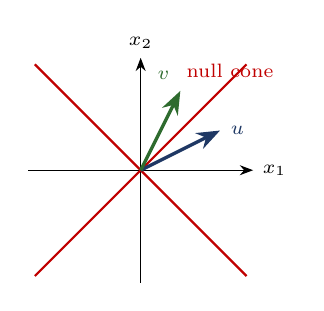
\begin{tikzpicture}[scale=0.42,>=Stealth]
        \draw[->] (-3.4,0) -- (3.4,0) node[right] {\scriptsize $x_1$};
        \draw[->] (0,-3.4) -- (0,3.4) node[above] {\scriptsize $x_2$};
        \draw[accent, thick] (-3.2,-3.2) -- (3.2,3.2);
        \draw[accent, thick] (-3.2,3.2) -- (3.2,-3.2);
        \draw[->, very thick, ink] (0,0) -- (2.4,1.2) node[right] {\scriptsize $u$};
        \draw[->, very thick, greenink] (0,0) -- (1.2,2.4) node[above left] {\scriptsize $v$};
        \node[accent, font=\scriptsize] at (2.7,3.0) {null cone};
      \end{tikzpicture}
    \end{center}
    库内资产：\texttt{artin-algebra-2e-ch08-ex-4.4-indefinite-orthogonality}（独立 TikZ 构造，非原书裁图）。
  \end{exampleblock}
\end{frame}

\begin{frame}[t]{三、Systematic Progress：LA214}
  \leavevmode\ex{LA214 · Ch.~8 §4 Ex.~4.5 · printed p.~254 / PDF p.~266 · intermediate}
  \pdfbookmark[2]{LA214 · Ch.8 S 4 Ex~4.5}{bm:la214}
  \begin{block}{\footnotesize 题面}
    \scriptsize Find an orthogonal basis for the form on $\mathbb R^n$ whose matrix is (a)~$\begin{pmatrix}1&1\\1&1\end{pmatrix}$, (b)~$\begin{pmatrix}1&0&1\\0&2&1\\1&1&1\end{pmatrix}$.
  \end{block}
  \begin{exampleblock}{\footnotesize 思路：(a) 核中向量与一切正交；(b) 用 $e_1,e_2$ 起步对 $e_3$ 正交化}
    \scriptsize
    \textbf{(a)} 取 $v_1=(1,0)^{\mathsf T}$，$v_2=(1,-1)^{\mathsf T}$。矩阵把 $v_2$ 送到 $0$，故
    $$(v_1,v_2)=v_1^{\mathsf T}Av_2=0,\qquad (v_2,v_2)=0,$$
    两向量无关，是正交基；对角型 $\operatorname{diag}(1,0)$（退化：允许零平方长度）。\\[2pt]
    \textbf{(b)} 取 $v_1=e_1$，$v_2=e_2$，$v_3=(-2,-1,2)^{\mathsf T}$。直接计算
    $$Av_3=(0,0,-1)^{\mathsf T}\ \Longrightarrow\ v_1^{\mathsf T}Av_3=v_2^{\mathsf T}Av_3=0,\qquad v_1^{\mathsf T}Av_2=A_{12}=0,$$
    平方长度
    $$(v_1,v_1)=1,\qquad (v_2,v_2)=2,\qquad (v_3,v_3)=v_3^{\mathsf T}Av_3=-2,$$
    对角型 $\operatorname{diag}(1,2,-2)$，符号差 $(2,1)$。$\square$
  \end{exampleblock}
  \begin{block}{\footnotesize 验算（NumPy 通过）}
    \scriptsize 程序验证两组基的 Gram 矩阵分别为 $\operatorname{diag}(1,0)$ 与 $\operatorname{diag}(1,2,-2)$。
  \end{block}
\end{frame}

\begin{frame}[t]{三、Systematic Progress：LA215}
  \leavevmode\ex{LA215 · Ch.~8 §4 Ex.~4.6 · printed p.~254 / PDF p.~266 · beginner}
  \pdfbookmark[2]{LA215 · Ch.8 S 4 Ex~4.6}{bm:la215}
  \begin{block}{\footnotesize 题面}
    \scriptsize Extend the vector $X_1=\frac12(1,-1,1,1)^{\mathsf T}$ to an orthonormal basis for $\mathbb R^4$.
  \end{block}
  \begin{exampleblock}{\footnotesize 思路：Hadamard 型 $\pm\frac12$ 符号模式}
    \scriptsize
    一个扩张为
    $$X_1=\tfrac12(1,-1,1,1)^{\mathsf T},\quad X_2=\tfrac12(1,1,-1,1)^{\mathsf T},\quad X_3=\tfrac12(1,1,1,-1)^{\mathsf T},\quad X_4=\tfrac12(1,-1,-1,-1)^{\mathsf T}.$$
    每个向量平方长度 $4\cdot(1/2)^2=1$。比较符号模式：任意两个不同向量恰在两个坐标同号、两个坐标异号，故内积为
    $$\tfrac14(1+1-1-1)=0.$$
    于是四向量两两正交且单位长，构成 $\mathbb R^4$ 的正交归一基。$\square$
  \end{exampleblock}
  \begin{block}{\footnotesize 验算（NumPy 通过）与结构}
    \scriptsize 程序验证 $X^{\mathsf T}X=I_4$。以这些为列的 $4\times4$ 矩阵是正交矩阵（Hadamard 型符号阵）；这类构造与 LA210 的求逆公式衔接。
  \end{block}
\end{frame}

\begin{frame}[t]{三、Systematic Progress：LA216}
  \leavevmode\ex{LA216 · Ch.~8 §4 Ex.~4.7 · printed p.~255 / PDF p.~267 · intermediate}
  \pdfbookmark[2]{LA216 · Ch.8 S 4 Ex~4.7}{bm:la216}
  \begin{block}{\footnotesize 题面}
    \scriptsize Apply the Gram--Schmidt procedure to the basis $(1,1,0)^{\mathsf T}$, $(1,0,1)^{\mathsf T}$, $(0,1,1)^{\mathsf T}$ of $\mathbb R^3$.
  \end{block}
  \begin{exampleblock}{\footnotesize 思路：逐步减投影，中间向量可约去非零标量}
    \scriptsize
    记 $v_1=(1,1,0)$，$v_2=(1,0,1)$，$v_3=(0,1,1)$。
    $$e_1=\frac{v_1}{\lVert v_1\rVert}=\frac{(1,1,0)^{\mathsf T}}{\sqrt2};\qquad
      u_2=v_2-\frac{v_1\cdot v_2}{v_1\cdot v_1}v_1=\tfrac12(1,-1,2)^{\mathsf T}\ \Rightarrow\ e_2=\frac{(1,-1,2)^{\mathsf T}}{\sqrt6};$$
    $$u_3=v_3-(v_3\cdot e_1)e_1-(v_3\cdot e_2)e_2=\tfrac23(-1,1,1)^{\mathsf T}\ \Rightarrow\ e_3=\frac{(-1,1,1)^{\mathsf T}}{\sqrt3}.$$
    程序验证三向量成正交归一基（NumPy 通过）；中间向量乘非零标量不改变最终方向。
  \end{exampleblock}
\end{frame}

\begin{frame}[t]{三、Systematic Progress：LA217}
  \leavevmode\ex{LA217 · Ch.~8 §4 Ex.~4.8 · printed p.~255 / PDF p.~267 · intermediate}
  \pdfbookmark[2]{LA217 · Ch.8 S 4 Ex~4.8}{bm:la217}
  \begin{block}{\footnotesize 题面}
    \scriptsize Let $A=\begin{pmatrix}2&1\\1&2\end{pmatrix}$. Find an orthonormal basis for $\mathbb R^2$ with respect to the form $X^{\mathsf T}AY$.
  \end{block}
  \begin{exampleblock}{\footnotesize 思路：用 $A$-内积做 Gram--Schmidt}
    \scriptsize
    首先 $(e_1,e_1)_A=e_1^{\mathsf T}Ae_1=2$，故
    $$u_1=\frac1{\sqrt2}(1,0)^{\mathsf T}.$$
    对 $e_2$ 消去 $A$-投影（$(e_1,e_2)_A=A_{12}=1$）：
    $$e_2-\frac{(e_1,e_2)_A}{(e_1,e_1)_A}e_1=e_2-\frac12e_1=\frac12(-1,2)^{\mathsf T}.$$
    计算 $(-1,2)A(-1,2)^{\mathsf T}=6$（即 $(-1,2)\cdot A(-1,2)^{\mathsf T}=(-1,2)\cdot(0,3)^{\mathsf T}=6$），故 $A$-正交归一基为
    $$\boxed{u_1=\frac1{\sqrt2}(1,0)^{\mathsf T},\qquad u_2=\frac1{\sqrt6}(-1,2)^{\mathsf T}},\qquad u_i^{\mathsf T}Au_j=\delta_{ij}.\ \square$$
  \end{exampleblock}
  \begin{block}{\footnotesize 验算（NumPy 通过）与前提}
    \scriptsize 程序验证 $U^{\mathsf T}AU=I$。$A$ 的顺序主子式为 $2,3$，正定，保证每步可归一化。
  \end{block}
\end{frame}

\begin{frame}[t]{三、Systematic Progress：LA218}
  \leavevmode\ex{LA218 · Ch.~8 §4 Ex.~4.9 · printed p.~255 / PDF p.~267 · intermediate}
  \pdfbookmark[2]{LA218 · Ch.8 S 4 Ex~4.9}{bm:la218}
  \begin{block}{\footnotesize 题面}
    \scriptsize Find an orthonormal basis for the space $P$ of real polynomials of degree $\le2$, with $(f,g)=\int_{-1}^1f(x)g(x)\,dx$.
  \end{block}
  \begin{exampleblock}{\footnotesize 思路：对 $1,x,x^2$ 做 Gram--Schmidt，利用奇偶性}
    \scriptsize
    $\lVert1\rVert^2=\int_{-1}^1dx=2$，故 $p_0=\tfrac1{\sqrt2}$。由奇偶性，$x$ 与 $1$、$x^2$ 都正交，且
    $$\lVert x\rVert^2=\int_{-1}^1x^2dx=\frac23\ \Longrightarrow\ p_1=\sqrt{\tfrac32}\,x.$$
    $x^2$ 在常数上的投影为 $\tfrac{\int x^2}{\int1}=\tfrac13$，取 $u_2=x^2-\tfrac13$，则 $\int_{-1}^1\big(x^2-\tfrac13\big)^2dx=\tfrac25-\tfrac49+\tfrac29=\tfrac8{45}$。故正交归一基为
    $$\boxed{\frac1{\sqrt2},\qquad \sqrt{\frac32}\,x,\qquad \sqrt{\frac58}\,(3x^2-1)},$$
    即前三个归一化 Legendre 多项式。$\square$
  \end{exampleblock}
  \begin{block}{\footnotesize 验算（NumPy 数值积分通过）与正定性}
    \scriptsize 程序验证三者 Gram 矩阵为 $I$。型正定：非零多项式不能在区间上几乎处处为零。
  \end{block}
\end{frame}

\begin{frame}[t]{三、Systematic Progress：LA219}
  \leavevmode\ex{LA219 · Ch.~8 §4 Ex.~4.10 · printed p.~255 / PDF p.~267 · beginner}
  \pdfbookmark[2]{LA219 · Ch.8 S 4 Ex~4.10}{bm:la219}
  \begin{block}{\footnotesize 题面}
    \scriptsize Let $V$ be the real $n\times n$ matrices. Prove $(A,B)=\operatorname{trace}(A^{\mathsf T}B)$ is a positive definite bilinear form and find an orthonormal basis.
  \end{block}
  \begin{exampleblock}{\footnotesize 思路：迹 = 元素对应乘积之和；矩阵单位本身正交归一}
    \scriptsize
    逐元素展开：
    $$\operatorname{trace}(A^{\mathsf T}B)=\sum_{i,j}a_{ij}b_{ij},$$
    右端显然实双线性、对称，且
    $$(A,A)=\sum_{i,j}a_{ij}^2>0\qquad(A\ne0),$$
    故正定（Frobenius 内积）。对矩阵单位 $(E_{ij},E_{kl})=\operatorname{trace}(E_{ji}E_{kl})=\delta_{ik}\delta_{jl}$，故 $\boxed{\{E_{ij}:1\le i,j\le n\}}$ 是现成的正交归一基，维数 $n^2$。$\square$
  \end{exampleblock}
  \begin{block}{\footnotesize 对照}
    \scriptsize 复矩阵上相应的 Hermite 型为 $\operatorname{trace}(A^*B)$，见 LA222(a)；迹的符号差问题见 LA221。
  \end{block}
\end{frame}

\begin{frame}[t]{三、Systematic Progress：LA221}
  \leavevmode\ex{LA221 · Ch.~8 §4 Ex.~4.12 · printed p.~255 / PDF p.~267 · advanced}
  \pdfbookmark[2]{LA221 · Ch.8 S 4 Ex~4.12}{bm:la221}
  \begin{block}{\footnotesize 题面}
    \scriptsize Let $V=\mathbb R^{2\times2}$. (a)~Matrix of $(A,B)=\operatorname{trace}(AB)$ in the basis $\{E_{ij}\}$; (b)~its signature; (c)~an orthogonal basis; (d)~signature of $\operatorname{trace}(AB)$ on $\mathbb R^{n\times n}$.
  \end{block}
  \begin{exampleblock}{\footnotesize 思路：$\operatorname{trace}(E_{ij}E_{kl})=\delta_{jk}\delta_{il}$；把 $E_{ij},E_{ji}$ 换成对称/反对称组合}
    \scriptsize
    \textbf{(a)} 在有序基 $(E_{11},E_{12},E_{21},E_{22})$ 下
    $$G=\begin{pmatrix}1&0&0&0\\0&0&1&0\\0&1&0&0\\0&0&0&1\end{pmatrix}.$$
    \textbf{(b)(c)} 基 $E_{11},\ E_{22},\ E_{12}+E_{21},\ E_{12}-E_{21}$ 正交，对角值
    $$\operatorname{tr}(E_{11}^2)=1,\quad \operatorname{tr}(E_{22}^2)=1,\quad \operatorname{tr}\big((E_{12}+E_{21})^2\big)=2,\quad \operatorname{tr}\big((E_{12}-E_{21})^2\big)=-2,$$
    符号差 $\boxed{(3,1)}$。\\
    \textbf{(d)} 对角单位给 $n$ 个正方向；每对 $i<j$ 给一正一负：$p=n+\binom n2=\frac{n(n+1)}2$，$m=\binom n2=\frac{n(n-1)}2$，$p+m=n^2$（非退化）。$\square$
  \end{exampleblock}
  \begin{block}{\footnotesize 验算（NumPy 通过）与结构}
    \scriptsize 正/负子空间恰为对称/反对称矩阵空间。
  \end{block}
\end{frame}

\begin{frame}[t]{三、Systematic Progress：LA222}
  \leavevmode\ex{LA222 · Ch.~8 §4 Ex.~4.13 · printed p.~255 / PDF p.~267 · advanced}
  \pdfbookmark[2]{LA222 · Ch.8 S 4 Ex~4.13}{bm:la222}
  \begin{block}{\footnotesize 题面}
    \scriptsize (a)~Does $(A,B)=\operatorname{trace}(A^*B)$ define a Hermitian form on $\mathbb C^{n\times n}$? If so, determine its signature. (b)~Same question for $(A,B)=\operatorname{trace}(AB)$.
  \end{block}
  \begin{exampleblock}{\footnotesize 思路：(a) 逐元素展开验证公理；(b) 检验第一变元的共轭线性}
    \scriptsize
    \textbf{(a)}
    $$\operatorname{trace}(A^*B)=\sum_{i,j}\overline{a_{ij}}b_{ij},$$
    对 $A$ 共轭线性、对 $B$ 线性，且 $(B,A)=\overline{(A,B)}$；又 $(A,A)=\sum_{i,j}|a_{ij}|^2>0$（$A\ne0$），故是正定 Hermite 型（复 Frobenius 内积）。复维数 $n^2$，符号差 $\boxed{(n^2,0)}$。\\[2pt]
    \textbf{(b)} $\operatorname{trace}(AB)$ 对两变元都是复线性的；检验共轭线性：
    $$\operatorname{trace}((iA)B)=i\operatorname{trace}(AB),$$
    而 Hermite 型要求因子 $\overline i=-i$。故不是 Hermite 型，没有 Hermite 符号差。$\square$
  \end{exampleblock}
  \begin{block}{\footnotesize 对照}
    \scriptsize 与 LA221 的实迹型 $\operatorname{trace}(AB)$（符号差 $(\tfrac{n(n+1)}2,\tfrac{n(n-1)}2)$）形成对照：换成 $A^*$ 后不定型变成正定型。
  \end{block}
\end{frame}

% ============================================================ 四、速查表
\begin{frame}[t]{四、42 题速查表（1/2）：Random Review}
  \label{sec:answers}
\pdfbookmark[1]{四、速查表}{bm:sec-answers}
  \centering\scriptsize
  \setlength{\tabcolsep}{3.2pt}
  \renewcommand{\arraystretch}{0.95}
  \begin{tabular}{@{}l l l@{}}
    \toprule
    题 & 定位 & 一句话结论\\
    \midrule
    F28 & Ch.~3 \S1 Ex.~1.1 & $a+b\sqrt2$ 成域；逆元 $=\frac{a-b\sqrt2}{a^2-2b^2}$\\
    LA163 & Ch.~5 \S1 Ex.~1.1 & Rodrigues 公式给出三个旋转矩阵（(b) 为循环置换阵）\\
    LA148 & Ch.~4 \S7 Ex.~7.4 & (a) 6 个组合；(b) 原书误印 $2$，意图 $J_2(-2)\oplus J_2(5)\oplus[5]$\\
    LA97 & Ch.~3 \S6 Ex.~6.3 & 尾段 $|a_i|\le1$ 给包含；$a_i=i^{-1/p}$ 给严格\\
    LA140 & Ch.~4 \S6 Ex.~6.7 & $A^{-1}(AB)A=BA$\\
    LA158 & Ch.~4 M.5 & 右逆 $\Leftrightarrow$ 满 $\Leftrightarrow$ 秩 $m$；左逆 $\Leftrightarrow$ 单 $\Leftrightarrow$ 秩 $n$\\
    LA118 & Ch.~4 \S4 Ex.~4.3 & 和与交的元素逐个检验不变性\\
    F29 & Ch.~3 \S1 Ex.~1.10 & $A^2=A+I$，$A^3=I$；$\cong\mathbb F_2[x]/(x^2+x+1)$\\
    LA77 & Ch.~3 \S2 Ex.~2.1 & $0v=0$ 消去；$-w=(-1)w\in W$\\
    LA183 & Ch.~5 \S4 Ex.~4.8 & $\|P^{-1}(B_k-B)P\|\le\|P^{-1}\|\|B_k-B\|\|P\|\to0$\\
    LA167 & Ch.~5 \S1 Ex.~1.5 & $\operatorname{rank}M=2$；轴向 $(a_{32}{-}a_{23},\,a_{13}{-}a_{31},\,a_{21}{-}a_{12})^t$\\
    LA93 & Ch.~3 \S5 Ex.~5.2 & $W_2=\mathbb RI$，迹投影分解\\
    LA149 & Ch.~4 \S7 Ex.~7.5 & 单特征线 $\Rightarrow J_n(\lambda)$（要求特征多项式分裂）\\
    LA105 & Ch.~4 \S1 Ex.~1.3 & $\dim\ker A=n-\operatorname{rank}A\ge n-m$\\
    LA90 & Ch.~3 \S4 Ex.~4.4 & $(p^2-1)(p^2-p)$；$|SL_2|=$ 其 $\tfrac1{p-1}$\\
    G182 & Ch.~6 \S12 Ex.~12.2 & 三轨道 $6+8+12$，稳定子阶 $4,3,2$\\
    LA79 & Ch.~3 \S3 Ex.~3.1 & $\{E_{ii}\}\cup\{E_{ij}+E_{ji}\}$，维数 $\tfrac{n(n+1)}2$\\
    G190 & Ch.~6 M.4 & $G_n=C_2^n\rtimes S_n$，$|G_n|=2^nn!$；$G_2\cong D_4$\\
    LA134 & Ch.~4 \S6 Ex.~6.1 & 比对 $t^{n-1}$ 系数与常数项\\
    LA145 & Ch.~4 \S7 Ex.~7.1 & $N=A-I$ 秩 1 平方零 $\Rightarrow J_2(1)\oplus[1]$\\
    G152 & Ch.~6 \S6 Ex.~6.5 & 三角格；$C_6\mapsto p6$，$D_6\mapsto p6m$\\
    \bottomrule
  \end{tabular}
\end{frame}

\begin{frame}[t]{四、42 题速查表（2/2）：Systematic Progress}
  \centering\fontsize{6.9}{8.1}\selectfont
  \setlength{\tabcolsep}{2.5pt}
  \renewcommand{\arraystretch}{0.86}
  \begin{tabular}{@{}l l l@{}}
    \toprule
    题 & 定位 & 一句话结论\\
    \midrule
    LA202 & \S2 Ex.~2.1 & $|a_{ij}|<\sqrt{a_{ii}a_{jj}}\le\max$ 对角元\\
    LA203 & \S2 Ex.~2.2 & 合同保秩（乘可逆矩阵）\\
    LA204 & \S3 Ex.~3.1 & 是：极化迫使反 Hermite 部分为零\\
    LA205 & \S3 Ex.~3.2 & 实部对称正定、虚部反对称\\
    LA206 & \S3 Ex.~3.3 & $\{E_{ii},E_{ij}+E_{ji},i(E_{ij}-E_{ji})\}$，维数 $n^2$\\
    LA207 & \S3 Ex.~3.4 & $(A^*A)^*=A^*A$；$X^*A^*AX=\lVert AX\rVert^2>0$\\
    LA208 & \S3 Ex.~3.5 & $A^2,A^{-1},A+B$ 是；$AB$ 不必然（$(AB)^*=BA$）\\
    LA209 & \S3 Ex.~3.6 & 判别式 $(a-d)^2+4|z|^2\ge0$\\
    LA210 & \S4 Ex.~4.1 & $P^{-1}=D^{-1}P^{\mathsf T}$，$D=P^{\mathsf T}P$ 对角\\
    LA211 & \S4 Ex.~4.2 & $\pi(x)=x-\frac{(v,x)}{(v,v)}v$（需 $(v,v)\ne0$）\\
    LA212 & \S4 Ex.~4.3 & $\ker(A^{\mathsf T}A)=\ker A\Rightarrow$ 同秩；半正定\\
    LA213 & \S4 Ex.~4.4 & $(a,b)\mapsto(b,a)$ 正交；零锥自正交\\
    LA214 & \S4 Ex.~4.5 & (a) $\operatorname{diag}(1,0)$；(b) $\operatorname{diag}(1,2,-2)$\\
    LA215 & \S4 Ex.~4.6 & $\pm\frac12$ Hadamard 型四向量\\
    LA216 & \S4 Ex.~4.7 & $(1,1,0)/\sqrt2,\ (1,-1,2)/\sqrt6,\ (-1,1,1)/\sqrt3$\\
    LA217 & \S4 Ex.~4.8 & $(1,0)/\sqrt2,\ (-1,2)/\sqrt6$（$A$-正交）\\
    LA218 & \S4 Ex.~4.9 & Legendre：$1/\sqrt2,\ \sqrt{3/2}\,x,\ \sqrt{5/8}(3x^2-1)$\\
    LA219 & \S4 Ex.~4.10 & 迹 $=$ 元素内积；$\{E_{ij}\}$ 正交归一\\
    LA220 & \S4 Ex.~4.11 & 和的补 $=$ 补的交；$W\subset W^{\perp\perp}$；反包含\\
    LA221 & \S4 Ex.~4.12 & $2\times2$ 符号差 $(3,1)$；一般 $(n(n{+}1)/2,\ n(n{-}1)/2)$\\
    LA222 & \S4 Ex.~4.13 & (a) 正定 Hermite，$(n^2,0)$；(b) 复双线性，非 Hermite\\
    \bottomrule
  \end{tabular}
\end{frame}

% ============================================================ 五、方法卡
\begin{frame}[t]{五、方法卡：本周反复出现的五类工具}
\pdfbookmark[1]{五、方法卡}{bm:sec-methods}
  \begin{columns}[T,onlytextwidth]
    \begin{column}{0.49\textwidth}
      \begin{block}{\footnotesize 1. Jordan 型的「分拆 + 块数」读法}
        \scriptsize
        每个特征值的块大小构成其代数重数的分拆；特征空间维数 $=$ 块数。秩与幂零指数进一步约束：$N^2=0$ 时块 $\le2$，$\operatorname{rank}N=\sum(\text{size}-1)$（LA148，LA145，LA149）。
      \end{block}
      \begin{block}{\footnotesize 2. 正定性的「限制到子空间」与「配平方」}
        \scriptsize
        正定限制到任意子空间仍正定（LA202 的 $2\times2$ 主子式）；$X^*A^*AX=\lVert AX\rVert^2$ 是把二次型写成平方和的标准动作（LA207，LA212）。
      \end{block}
      \begin{block}{\footnotesize 3. Hermite $/$ 复分解}
        \scriptsize
        $A=H+iK$（$H,K$ Hermite）+ 在 $e_i,\ e_i+e_j,\ e_i+ie_j$ 上测试，是复极化的模板（LA204，LA205，LA222）。
      \end{block}
    \end{column}
    \begin{column}{0.49\textwidth}
      \begin{block}{\footnotesize 4. Gram--Schmidt 的三个变体}
        \scriptsize
        欧氏（LA216）、带权 $A$-内积（LA217）、积分内积（LA218：Legendre）。共同骨架：减去已得方向上的投影，再归一化；中间向量可约去公共标量。
      \end{block}
      \begin{block}{\footnotesize 5. 群作用的「轨道--稳定子」计数}
        \scriptsize
        先找几何类型，再验证传递性，最后 $|G|/|G_v|$ 核对规模（G182 的 $6,8,12$；G190 的 $2^n$ 顶点与 $2^nn!$ 阶；LA90 的 $|GL_2|,\ |SL_2|$）。
      \end{block}
      \begin{exampleblock}{\footnotesize 程序验算范围（NumPy，14 项全部通过）}
        \scriptsize
        LA163(b)(c)、LA145、LA90（$p=2,3,5$ 穷举）、LA208、LA214(a)(b)、LA215、LA216、LA217、LA218（数值积分）、LA221、F29（模 2）、LA148（特征根）。解析证明仍以笔记内独立推导为准。
      \end{exampleblock}
    \end{column}
  \end{columns}
\end{frame}

% ============================================================ 六、易错点
\begin{frame}[t]{六、易错点与边界条件}
\pdfbookmark[1]{六、易错点}{bm:sec-pitfalls}
  \begin{columns}[T,onlytextwidth]
    \begin{column}{0.49\textwidth}
      \begin{alertblock}{\footnotesize 概念混淆}
        \scriptsize
        \begin{itemize}\setlength{\itemsep}{1pt}
          \item \textbf{合同 $\ne$ 相似}：$P^{\mathsf T}AP$ 保秩保符号差，$P^{-1}AP$ 保特征值（LA203）。
          \item \textbf{$AB$ 的伴随}：$(AB)^*=BA$，乘序反转；正定矩阵之积未必 Hermite（LA208）。
          \item \textbf{正交（不定型）}：Lorentz 平面里正交向量不在欧氏直角上，且存在自正交的非零向量（LA213）。
        \end{itemize}
      \end{alertblock}
      \begin{alertblock}{\footnotesize 隐藏前提}
        \scriptsize
        \begin{itemize}\setlength{\itemsep}{1pt}
          \item LA149 的 Jordan 结论要求特征多项式分裂（复矩阵场景）。
          \item LA211 投影公式要求 $(v,v)\ne0$；LA210 要求列非零。
          \item LA140 的相似性依赖 $A$ 可逆；LA77(b) 依赖子空间的标量闭包定义。
        \end{itemize}
      \end{alertblock}
    \end{column}
    \begin{column}{0.49\textwidth}
      \begin{alertblock}{\footnotesize 原书问题（不静默修改）}
        \scriptsize
        \begin{itemize}\setlength{\itemsep}{1pt}
          \item \textbf{LA148 (b)}：印刷本把 $-2$ 写成 $2$，与特征多项式 $(t+2)^2(t-5)^3$ 矛盾。字面读：无解（$2$ 不是根，特征空间为零）；意图读（$-2$）：唯一答案 $J_2(-2)\oplus J_2(5)\oplus[5]$。笔记与讲义均双读法报告。
        \end{itemize}
      \end{alertblock}
      \begin{block}{\footnotesize 记号提醒}
        \scriptsize
        \begin{itemize}\setlength{\itemsep}{1pt}
          \item $A^*$（共轭转置）vs $A^{\mathsf T}$（转置）：LA207/212/222 的平方和论证依赖前者。
          \item 迹型 $\operatorname{trace}(AB)$（不定）vs $\operatorname{trace}(A^*B)$（正定）：LA221 vs LA222。
          \item $\ell^p$ 的 $p$ 是求和指数，与域 $\mathbb F_p$ 的 $p$ 无关（LA97 vs LA90）。
        \end{itemize}
      \end{block}
    \end{column}
  \end{columns}
\end{frame}

% ============================================================ 七、自测
\begin{frame}[t]{七、自测：下周初快速回顾的十问}
\pdfbookmark[1]{七、自测}{bm:sec-selftest}
  \begin{columns}[T,onlytextwidth]
    \begin{column}{0.49\textwidth}
      \begin{exampleblock}{\footnotesize 问题（答案见对应帧）}
        \scriptsize
        \begin{enumerate}\setlength{\itemsep}{1pt}
          \item $(1+\sqrt2)^{-1}$ 写成 $a+b\sqrt2$ 的形式？（F28）
          \item $2\pi/3$ 绕 $(1,1,1)$ 的旋转矩阵作用在 $e_1$ 上得什么？（LA163）
          \item $(t+2)^2(t-5)^3$、$5$-特征空间二维、$-2$ 特征线一维时的 Jordan 型？（LA148）
          \item 举一个 $\ell^2\setminus\ell^1$ 的显式序列？（LA97）
          \item $SO_3$ 中如何从矩阵元素读出旋转轴？（LA167）
          \item $|GL_2(\mathbb F_7)|$ 等于多少？（LA90）
        \end{enumerate}
      \end{exampleblock}
    \end{column}
    \begin{column}{0.49\textwidth}
      \begin{exampleblock}{\footnotesize 问题（续）}
        \scriptsize
        \begin{enumerate}\setlength{\itemsep}{1pt}\setcounter{enumi}{6}
          \item 正定矩阵哪些运算保持正定 Hermite？哪个不保证？反例？（LA208）
          \item 列正交（非单位）矩阵的逆公式？（LA210）
          \item $\bigl(\begin{smallmatrix}2&1\\1&2\end{smallmatrix}\bigr)$-内积下 $\mathbb R^2$ 的正交归一基？（LA217）
          \item $\operatorname{trace}(AB)$ 在 $\mathbb R^{n\times n}$ 上的符号差？（LA221）
        \end{enumerate}
      \end{exampleblock}
      \begin{block}{\footnotesize 收尾}
        \scriptsize
        本讲义为派生快照：不改动任何笔记、状态或题单；下周系统区将从 Ch.~8 \S4 之后继续。速查表起于第 \pageref{sec:answers} 页。
      \end{block}
    \end{column}
  \end{columns}
\end{frame}

\end{document}
